\documentclass[11pt,a4paper]{article}
\usepackage[margin=0.92in]{geometry}
\usepackage[T1]{fontenc}
\usepackage[utf8]{inputenc}
\usepackage{lmodern,microtype}
\usepackage{amsmath,amssymb,amsthm,mathtools,bm}
\usepackage{booktabs,tabularx,array}
\usepackage{graphicx,xcolor}
\usepackage{tikz,pgfplots}
\pgfplotsset{compat=1.18}
\usepackage[colorlinks=true,linkcolor=blue!55!black,citecolor=blue!55!black,urlcolor=blue!55!black]{hyperref}
\usepackage{cleveref,enumitem}
\definecolor{navy}{HTML}{17324D}
\definecolor{teal}{HTML}{167D89}
\definecolor{rose}{HTML}{B34A54}
\definecolor{slate}{HTML}{586576}
\newtheorem{proposition}{Proposition}
\newtheorem{theorem}{Theorem}
\newtheorem{remark}{Remark}
\newcommand{\pos}[1]{(#1)^+}
\newcommand{\CP}{\mathrm{CP}}
\newcommand{\CL}{\mathrm{CL}}
\newcommand{\DL}{\mathrm{DL}}
\newcommand{\E}{\mathbb{E}}
\newcommand{\Q}{\mathbb{Q}}
\newcommand{\lvr}{\mathrm{LVR}}
\title{\bfseries\color{navy}Option-Lot-Constrained Hedging of Automated Market Maker Liquidity:\\Certified Static Error Bounds and Empirical Order-Book Costs}
\author{Research manuscript --- authors to be determined\\
\small Reproducible study from the \texttt{arbitage} repository}
\date{Historical market data: October 9, 2026 \quad|\quad Draft version 1}
\begin{document}
\maketitle
\vspace{-1em}
\begin{abstract}
Concentrated automated market maker (AMM) positions expose liquidity providers to short convexity that admits static representation by European option payoffs. Existing work established the replication perspective, yet unrestricted continuous-strike portfolios may violate exchange strike grids, contract increments, available order-book depth and execution budgets. We combine constant-product (CPMM), concentrated (CLMM) and discretized liquidity (DLMM) models with Solana and Ethereum pool observations and contemporaneous Deribit option quotes. We give an interpolation error bound for smooth convexity, an obstruction to hedging isolated discrete Bin kinks with coarse option lots, and a mixed-integer minimax hedge evaluated by an exact continuous-price residual oracle. A saved \$10,000 hypothetical Solana DLMM position requires three 10-SOL option lots costing about \$123 to reduce its certified maximum absolute nonlinear residual over a $\pm10\%$ terminal price window from \$202.45 to \$29.46. Further SOL and ETH cases show substantial heterogeneity across AMM concentration and exchange lot sizes. Public on-chain Bin-fee observations are studied separately and do not establish profitable LP returns. The empirical contribution is therefore a reproducible \emph{hedging feasibility} analysis, not an executed arbitrage or investment-performance claim.
\end{abstract}
\noindent\textbf{Keywords:} automated market maker; option replication; integer optimization; impermanent loss; robust hedging; order-book depth; decentralized finance.
\section{Introduction}
Liquidity provision in an automated market maker exchanges directional inventory exposure and adverse selection for swap fees. The value of a passive liquidity position is normally concave in the outside-market asset price, corresponding to a short-convexity profile. Milionis et al.\ formalize loss-versus-rebalancing (LVR) and its connection to arbitrage against stale AMM prices \cite{milionis2022lvr,milionis2023fees}. European-option representations of impermanent loss, including concentrated liquidity, are already known \cite{deng2023static}. We do \emph{not} treat option replication as a novel insight.

Our question is operationally narrower: for a fixed, hypothetical LP payoff, what risk reduction is possible \emph{with listed} European options when order size comes in discrete contract increments, the strike set is sparse, ask-side depth is limited, and premiums are paid? Unconstrained replication at every Bin strike does not imply an executable hedge.

Our research contributions are:
\begin{enumerate}[leftmargin=*,itemsep=2pt]
\item A common initial-HODL-relative loss model for full-range CPMM, bounded CLMM and discrete fixed-Bin DLMM, explicitly distinct from directional principal loss and pathwise LVR.
\item A smooth spline error upper bound and an elementary but nonzero \emph{local lot-quantization error lower bound} for isolated DLMM kinks. They characterize why theoretical zero-error replication may not be accessible to small investors.
\item An integer cost-versus-worst-residual formulation with a continuous-price residual-risk oracle; the numerical study uses archived pool accounts, displayed Deribit ask ladders, realistic SOL and ETH contract increments, and separate on-chain fee-growth checks.
\end{enumerate}
The interpolation lemma and mixed-integer programming ingredients are standard; the contribution is their transparent integration into an explicitly bounded, real-market-data LP hedge exercise. The study does not assert novel no-arbitrage option pricing, profitable implementation, or global MILP optimality beyond reported solver gaps.

\subsection{Related research}
The LVR decomposition of \cite{milionis2022lvr} highlights arbitrage losses beyond naive end-to-end impermanent loss, while \cite{milionis2023fees} shows how trading fees change arbitrage incentives. Deng, Zong and Wang \cite{deng2023static} derive static replication formulas for concentrated impermanent loss. Protocol-specific LP fee accounting depends additionally on liquidity placement, swap routing and position checkpoints \cite{univ3,meteoraaccounts}. Our analysis deliberately studies a narrower terminal European option hedge and explicitly reports where empirical fees cannot be inferred from public total-value-locked data.

\section{A Common Terminal Risk Benchmark}
Let $S_0>0$ denote the entry price of a volatile token in USDC, and $W$ the entry value of an LP position. Let $x_0$ be the initial number of volatile units. The \emph{initial-token HODL} comparator is
\begin{equation}
B(S)=W+x_0(S-S_0).
\label{eq:hodl}
\end{equation}
For an idealized fee-free AMM whose inventory instantly follows a frictionless arbitrage-equilibrium value $V(S)$, define
\begin{equation}
 D(S)=B(S)-V(S),\qquad D(S_0)=0.
 \label{eq:divergence}
\end{equation}
The loss $D$ is \emph{relative to HODL}, not a dollar-capital loss. If SOL falls, $B(S)$ itself decreases; compensating $D$ does not eliminate that exposure. Real execution is path dependent; throughout the replication analysis, $D$ means \emph{fee-free terminal curvature only}.

\subsection{Constant-product market maker}
For a 50/50 deposit into a full-range pool $xy=k$,
\begin{align}
V_{\CP}(S)&=W\sqrt{S/S_0},&
x_0&=W/(2S_0),\label{eq:cp-value}\\
D_{\CP}(S)&=\frac{W}{2}\left(\sqrt{S/S_0}-1\right)^2,&
D_{\CP}''(S)&=\frac{W}{4\sqrt{S_0}S^{3/2}}>0.
\label{eq:cp-loss}
\end{align}
For example, if the pool begins at \$10,000, a terminal 10\% SOL decline causes only about \$13.17 of divergence from the initial same-token HODL basket, but the fee-free LP's \emph{dollar} value is approximately \$9,486.83. Full-range simplicity does not imply cash principal preservation.

\subsection{Finite-range concentrated liquidity}
Let $0<a<S_0<b$ be the concentrated position's range and $L>0$ its liquidity parameter. The inventories are
\begin{equation}
x(S)=\begin{cases}
L(a^{-1/2}-b^{-1/2}),&S\le a,\\
L(S^{-1/2}-b^{-1/2}),&a<S<b,\\
0,&S\ge b,
\end{cases}\qquad
y(S)=\begin{cases}
0,&S\le a,\\
L(\sqrt S-\sqrt a),&a<S<b,\\
L(\sqrt b-\sqrt a),&S\ge b.
\end{cases}
\label{eq:cl-inventory}
\end{equation}
Set $V_{\CL}(S)=Sx(S)+y(S)$, $x_0=x(S_0)$ and $W=V_{\CL}(S_0)$. In the active interval,
\begin{equation}
 V_{\CL}(S)=L\big(2\sqrt S-S/\sqrt b-\sqrt a\big),
 \qquad D_{\CL}''(S)=\frac{L}{2S^{3/2}},
\label{eq:cl-value}
\end{equation}
whereas $V_{\CL}$ is affine outside $[a,b]$. Narrower ranges generally concentrate more short curvature per invested dollar.

\subsection{Static idealized discrete-Bin inventory}
For fixed Bin conversion prices $K_i$, suppose lower Bins ($K_i<S_0$) initially contain $Y_i$ units of stable quotation asset and upper Bins initially contain $X_i$ volatile units. Under \emph{complete fee-free conversion at the Bin price}, omitting the mixed active Bin,
\begin{equation}
D_{\DL}(S)=
\sum_{K_i<S_0}\frac{Y_i}{K_i}(K_i-S)^+
+\sum_{K_i>S_0}X_i(S-K_i)^+.
\label{eq:dl-bins}
\end{equation}
The underlying curvature is atomic:
\begin{equation}
 D_{\DL}''=\sum_i q_i\delta_{K_i},\qquad
 q_i=\begin{cases}Y_i/K_i,&K_i<S_0,\\X_i,&K_i>S_0.\end{cases}
\label{eq:dl-atoms}
\end{equation}
Equation \eqref{eq:dl-bins} is an exact identity \emph{for this synthetic static conversion model}, not an exact realized Meteora PositionV2 cash-flow formula with dynamic fees, partial fills or rebalancing.

\subsection{Terminal divergence versus pathwise LVR}
For a continuously arbitraged, fee-free model, It\^o--Tanaka expresses the ideal DLMM LVR in terms of weighted semimartingale local times:
\begin{equation}
 \lvr_T^{\DL}=\frac12\sum_i q_i L_T^{K_i}(S).
\label{eq:local-time}
\end{equation}
An external-price round trip may generate positive LVR but zero \emph{terminal} divergence. Therefore the static European option analysis below hedges $D(S_T)$, not each pathwise source of adverse selection. Actual LP fees and dynamic inventory rebalance are not bundled into its hedge claims.

\section{Continuous Replication and Quantization Bounds}
Define put and call hinges $p_K(S)=(K-S)^+$ and $c_K(S)=(S-K)^+$. The ideal DLMM loss \eqref{eq:dl-bins} is already a finite portfolio of these European payoffs, provided that fractional quantities and \emph{all} Bin strikes are traded. For a sufficiently smooth convex loss, one similarly has a continuum-of-hinges representation up to an affine term. The existence of static impermanent-loss replication is not new \cite{deng2023static}; we isolate the precision lost when it must be discretized.

\begin{proposition}[Uniform interpolation upper bound]
\label{prop:spline}
Let $D\in C^2([a,b])$ be convex, with $0\le D''(S)\le M$. Let $I_hD$ be the continuous piecewise-affine interpolant through nodes $a=s_0<\cdots<s_N=b$ of maximum spacing $h$. Then
\begin{equation}
 0\le I_hD(S)-D(S)\le\frac{Mh^2}{8},\qquad
 S\in[a,b].
\label{eq:interpolation}
\end{equation}
Furthermore $I_hD$ is an affine function plus a portfolio of hinge payoffs with nonnegative slope jumps.
\end{proposition}
\begin{proof}
Fix $[s_j,s_{j+1}]$ and write $E=I_hD-D$. It vanishes at the endpoints and satisfies $-M\le E''\le0$. Comparing $E$ with the quadratic barrier $\tfrac M2(S-s_j)(s_{j+1}-S)$ proves the upper bound, with maximum $M(s_{j+1}-s_j)^2/8$ at the midpoint. Convexity gives $I_hD\ge D$. The secant slopes of $D$ are nondecreasing, so adjacent affine segments have nonnegative derivative jumps representable by call hinges (or a put/call decomposition relative to an anchor strike).
\end{proof}
For a uniform grid, $\varepsilon$ accuracy follows whenever $h\le\sqrt{8\varepsilon/M}$. This bound assumes arbitrary strike positions and \emph{fractional} hedge quantities, and hence is not a certificate for a listed-derivatives exchange.

\subsection{Minimum tradable option lots create an error floor}
Let $m>0$ be the smallest underlying-asset quantity of a particular listed option contract. An AMM kink of size $q$ at strike $K$ can be matched exactly only when $q$ is in $m\mathbb{Z}_{\ge0}$, unless additional instruments or a more complicated offset are permitted.

\begin{proposition}[Local lot-quantization obstruction]
\label{prop:obstruction}
Suppose $D$ is continuous and piecewise affine on $[K-h,K+h]$, with precisely one interior derivative jump $q>0$ at $K$. Suppose that the hedge has derivative jump $nm$ at $K$ for integer $n\ge0$, and no other target or hedge strikes lie in the open interval. For residual $R=D-H$, any affine correction satisfies
\begin{equation}
\|R\|_{\infty,[K-h,K+h]}
 \ge\frac h4|q-nm|.
\label{eq:quant-bound}
\end{equation}
Taking the best integer quantity gives a bound of
$\frac h4\operatorname{dist}(q,m\mathbb Z_{\ge0})$.
\end{proposition}
\begin{proof}
The residual $R$ is affine separately on both sides of $K$, with slope change $\delta=q-nm$. The symmetric second finite difference is
\[
R(K-h)-2R(K)+R(K+h)=h\delta.
\]
Its absolute value is at most $4\|R\|_\infty$, giving \eqref{eq:quant-bound}. An affine correction drops out of the second finite difference.
\end{proof}
The assumptions deliberately exclude nearby unmatched strikes: the statement is a local \emph{DLMM kink} result, not a universal residual lower bound for smooth CPMMs or arbitrary option portfolios. It reveals a scale effect. If a hypothetical LP allocation is multiplied by capital $W$, its kink quantity is $q(W)=Wq(1)$, while venue contract increments stay fixed. The mismatch $|Wq(1)-nm|$ changes in discrete steps rather than proportionally with $W$. Consequently there is \emph{no universal requirement} to deposit \$10,000 before an LP can be hedged; the useful account size depends on its risk concentration, available option contracts, and acceptable error.

\subsection{Premium is an economic counterpart to negative convexity}
The risk-neutral expectation of \eqref{eq:dl-bins}, when well defined, is a sum of vanilla option prices. Even perfect fee-free replication generally costs money. Under a zero-interest, risk-neutral geometric Brownian model with constant volatility $\sigma$ and $T$ in years, the idealized full-range CPMM expectation is
\begin{equation}
\E^{\Q}\left[D_{\CP}(S_T)\right]
=W\left(1-\exp\left\{-\frac{\sigma^2T}{8}\right\}\right).
\label{eq:cp-expected}
\end{equation}
Indeed, if $r=S_T/S_0$, then $\E^\Q[r]=1$ and $\E^\Q[\sqrt r]=\exp(-\sigma^2T/8)$. This is a \emph{risk-neutral convexity valuation}, not the physical expectation of future losses, and actual option ask premiums include spread and market microstructure.

\section{Hedging with Finite Strikes, Lots and Ask-Side Depth}
Fix a positive terminal stress interval $\mathcal I=[S_-,S_+]$. Each available option $j$ is specified by type $\tau_j\in\{p,c\}$, strike $K_j$, underlying asset size per exchange lot $m_j$, displayed ask-depth capacity $N_j$, and a price ladder. With the integer number of lots $n_j$ and payoff hinge $h_{\tau_j,K_j}\in\{p_{K_j},c_{K_j}\}$, the long-only terminal protection is
\begin{equation}
 H_{\bm n}(S)=\sum_{j=1}^J n_jm_jh_{\tau_j,K_j}(S),
 \qquad n_j\in\{0,\ldots,N_j\}.
\label{eq:hedge}
\end{equation}
Write $C(\bm n)$ for \emph{indicative} ask-ladder premiums plus a modeled fee budget. The depth ladder can be expanded into binary/integer variables with precedence constraints: a more expensive ask level may be used only after the cheaper displayed level is exhausted. This is an execution \emph{estimate}; a book snapshot cannot guarantee the quoted sizes will still be there when the orders arrive.

For a risk-weight $\lambda\ge0$, we optimize
\begin{equation}
\begin{aligned}
 \min_{\bm n,z}\quad&C(\bm n)+\lambda z\\
 \text{subject to}\quad&
   -z\le D(S)-H_{\bm n}(S)\le z
      &&\forall S\in\mathcal I,\\
 &n_j\in\mathbb{Z}_{\ge0},\quad 0\le n_j\le N_j.
\end{aligned}
\label{eq:minimax}
\end{equation}
The quantity $z$ is the \emph{worst absolute nonlinear terminal residual}. It is neither an expected return nor a loss bound for the LP's total dollar principal. The explicit loss of the dollar price sensitivity from the initial portfolio, as well as the effect of funding and fee compounding, remain outside this optimization.

\begin{theorem}[Continuous-price exact error oracle]
\label{thm:exact}
For the CPMM, CLMM and finite idealized DLMM loss functions in \cref{eq:cp-loss,eq:cl-value,eq:dl-bins}, and for any fixed finite listed-option portfolio \eqref{eq:hedge}, the maximum of $|D-H_{\bm n}|$ on the compact interval $\mathcal I$ is attained at one of the following points:
(i) an interval endpoint;
(ii) a strike, Bin, or CLMM range breakpoint within $\mathcal I$;
(iii) a stationary point of $D-H_{\bm n}$ inside a differentiable segment.
\end{theorem}
\begin{proof}
The residual is continuous and piecewise $C^2$, with finitely many structural breakpoints. On each closed smooth segment, a maximum of its absolute value occurs at an endpoint or at a point of zero derivative unless the residual vanishes identically. For CPMM, $D'=x_0-W/(2\sqrt{S_0S})$; for an active CLMM, $D'=x_0-L(S^{-1/2}-b^{-1/2})$. Between option strikes, $H_{\bm n}'$ is constant, so candidate stationary roots can be solved explicitly. For DLMM, $D-H_{\bm n}$ is affine between breakpoints, so no interior stationary evaluation is required except constant segments.
\end{proof}
An exact continuous-spot \emph{a posteriori} envelope does not by itself prove that the mixed-integer optimizer found a global minimum. The implementation uses cutting planes. It initializes a finite set of endpoints and kinks, solves the restricted mixed-integer linear program, evaluates \cref{thm:exact} independently, and adds any violated extremal price before resolving. The final risk estimate is reported independently of the MILP optimality gap.

\begin{remark}[Interpretation of the cost--risk objective]
At $\lambda=0.1$, a solution may rationally purchase zero contracts, while at $\lambda=1$ it can purchase many. These are \emph{risk-preference scenarios}; the paper does not calibrate them to observed investor utility. Even when $C+z$ is less than an assumed fee budget, execution risk, basis exposure, price beta, fees and exit costs make a profitability conclusion unwarranted.
\end{remark}

\section{Data and Reproducibility Design}
The empirical input consists of dated \emph{public} Solana and Ethereum AMM pool data, Meteora Bin inventory/fee-growth account snapshots, and displayed Deribit option ask ladders. Pool and option observations are \emph{not atomic}, and exact collection timestamps are preserved. We do not infer a live wallet position from a pool's aggregated Bin reserves. All source scripts, past run IDs and output summaries are available under the public \href{https://github.com/evaristebernhard/arbitage}{\texttt{arbitage} research repository}.

\paragraph{Meteora data and decimal audit.}
The SOL/USDC 4-bp Meteora pool
\texttt{5rCf1DM8...TogYHAS6} (full identifier in the machine-readable data manifest)
was snapshotted at 08:23:08 UTC on October 9, 2026, with active Bin ID $-5513$, 4,908 populated Bins and approximately \$4.006 million marked reserves. A previous snapshot collector had mistakenly applied SOL/USDC decimal conversion twice; the static optimizer checks the saved active Bin price against an independently saved pool price and corrects a factor 1,000 \emph{on reading}, leaving original archived data unmodified. This audit matters because false Bin strike prices would invalidate every hedge result. The option snapshot is from 08:23:52 UTC, 44.93 seconds later; its SOL index is \$110.2492 against pool mark \$110.2771.

\paragraph{SOL and ETH option units.}
All Solana tests use the SOL\_USDC October 23, 2026 expiration, at 08:00 UTC; the displayed minimum order increment in the collected SOL data is one whole \emph{10-SOL} option contract. Ethereum tests independently use ETH\_USDC options of the same expiration, with one full contract equal to \emph{1 ETH} but a \emph{minimum trading step of 0.1 ETH}. Quantities are normalized to underlying units before optimization. The two chains' spot prices, underlying option books and hedge positions are never mixed \cite{deribitlinear}.

\paragraph{Snapshot attribution.}
The main Meteora result comes from successful GitHub Actions run
\href{https://github.com/evaristebernhard/arbitage/actions/runs/37910170471}{37910170471}, whose JSON artifact records exact Bin counts, index basis, premiums, MILP gaps and stationary-breakpoint verification. A distinct SOL cross-protocol screen saved around 10:08 UTC supplies the Raydium full-range versus CLMM comparison; it is documented in \texttt{docs/sol-cross-protocol-option-screen-20261009.md}. A separate
\href{https://github.com/evaristebernhard/arbitage/actions/runs/37916764413}{ETH/Uniswap experiment (37916764413)}
has its own option quote timestamp, strike chain and underlying contract sizes. The short-run fee-counter study uses
\href{https://github.com/evaristebernhard/arbitage/actions/runs/37928429533}{run 37928429533} and refers to different on-chain times. Historical option-book snapshots are \emph{quotes}, not executed market trades or backtested fills.

\section{Empirical Hedge-Cost Frontiers}
Every experiment below uses a hypothetical initial LP principal of \$10,000. The core performance quantity $z$ is the \emph{largest absolute fee-free terminal convexity residual} over a chosen stress window, found by the independent continuous-price oracle. A residual of \$20 is not a maximum possible \$20 investment loss. The hedge is long-option-only; the integer solver is limited to observed ask depths and reports nonzero MILP gap when applicable.

\subsection{Meteora: real Bin reserves against SOL option asks}
For the Oct.\ 9 08:23 UTC 4-bp Meteora SOL/USDC snapshot, the entire pool's Bin inventories were scaled \emph{pro rata} to \$10,000 and used as a \emph{synthetic} cross-Bin LP basket. This collection of Bins does not establish any one user's actually mintable PositionV2 or fees. The risk objective \eqref{eq:minimax} was solved for each of two terminal stress windows and risk parameters.

\begin{table}[ht]
\centering
\caption{SOL DLMM Bin-inventory experiment with archived option ask ladder. $z_0$ is the unhedged worst absolute residual, $z$ the hedged worst residual. Option outlay includes indicative venue fees.}
\label{tab:dlmm}
\small
\begin{tabular}{@{}ccrrrr@{}}
\toprule
Spot window & $\lambda$ & SOL lots & Outlay (\$) & $z_0$ (\$) & $z$ (\$)\\
\midrule
$\pm10\%$ & 0.1 & 0 & 0.00 & 202.45 & 202.45\\
$\pm10\%$ & 1.0 & 3 & 122.99 & 202.45 & 29.46\\
$\pm20\%$ & 0.1 & 0 & 0.00 & 745.67 & 745.67\\
$\pm20\%$ & 1.0 & 7 & 177.32 & 745.67 & 15.83\\
\bottomrule
\end{tabular}
\end{table}

For $\pm10\%$ and $\lambda=1$, the selected hedge consists of one Oct.\ 23 strike-110 SOL put and one each of strike-111 and strike-114 SOL calls, each covering 10 SOL. The \emph{displayed premium} is \$122.00; \$122.99 includes the modeled trading fees. The bounded nonlinear risk $z$ falls from \$202.4546 to \$29.4555 over all terminal prices in the specified interval. The option cost \emph{plus} this absolute residual is \$152.45.

For the $\pm20\%$ window, the solver selects two puts (strikes 104 and 108) and five calls (113, 115, 118, 120 and 122), for a \$177.32 estimated outlay and \$15.83 maximum nonlinear residual. This is not a paradox: each stress window defines a different minimax objective and permits different hedge strikes, quantities, and levels of overhedging. The final reported MILP relative gaps are approximately 0.00366 and 0.00492. We claim the oracle's \emph{certified model residual}, not a proof of exactly optimal integer portfolios.

\subsection{The cost of concentrating SOL liquidity}
A separate Oct.\ 9 10:08 UTC Solana snapshot used its own SOL index and Deribit ask ladders to compare an idealized Raydium CPMM with constructed CLMM positions. All use $\pm10\%$ terminal stress and $\lambda=1$.

\begin{table}[ht]
\centering
\caption{Different hypothetical LP payoff geometries hedged using a distinct SOL option-book sample at 10:08 UTC, \$10,000 principal.}
\label{tab:sol}
\small
\begin{tabular}{@{}lrrrr@{}}
\toprule
LP configuration & Lots & Outlay (\$) & $z_0$ (\$) & $z$ (\$)\\
\midrule
Full-range CPMM & 0 & 0.00 & 13.17 & 13.17\\
CLMM $\pm2.5\%$ & 8 & 318.65 & 448.17 & 40.91\\
CLMM $\pm5.0\%$ & 8 & 279.65 & 392.56 & 25.30\\
CLMM $\pm10.0\%$ & 7 & 197.32 & 269.12 & 11.86\\
\bottomrule
\end{tabular}
\end{table}
The full-range model has considerably less \emph{HODL-relative} fee-free nonlinear loss under the prescribed 10\% terminal stress. It does not imply low spot beta or principal protection. An actual concentrated LP might earn more swap fees while in range; the corresponding owner-specific fee data are not part of this simultaneous option-book snapshot.

\begin{figure}[ht]
\centering
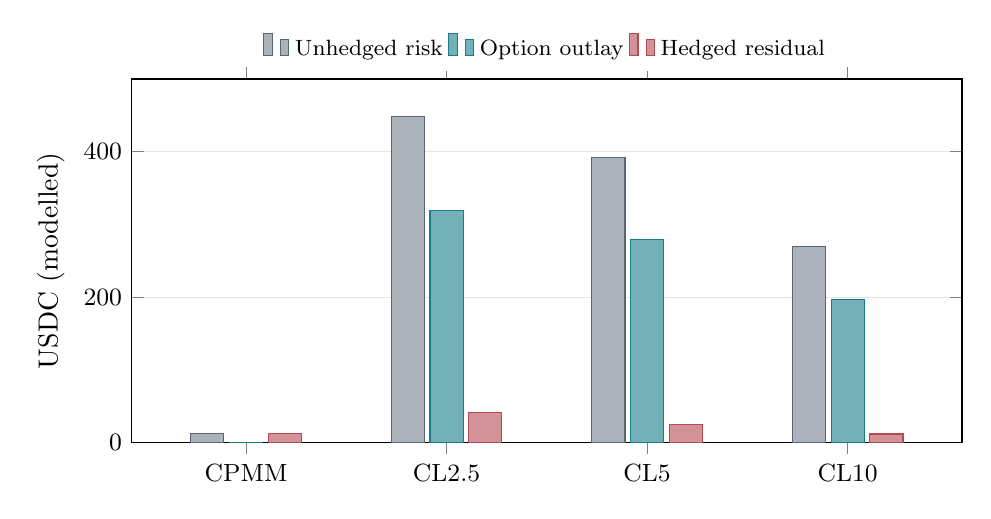
\begin{tikzpicture}
\begin{axis}[
  ybar,bar width=12pt,
  width=\linewidth,height=6.2cm,
  ymin=0,ymax=500,
  symbolic x coords={CPMM,CL2.5,CL5,CL10},
  xtick=data,
  ylabel={USDC (modelled)},
  tick label style={font=\small},
  legend style={at={(0.5,1.02)},anchor=south,legend columns=3,font=\footnotesize,draw=none},
  ymajorgrids=true,grid style={gray!20},
  enlarge x limits=0.19]
\addplot[fill=slate!50,draw=slate] coordinates {(CPMM,13.17)(CL2.5,448.17)(CL5,392.56)(CL10,269.12)};
\addplot[fill=teal!60,draw=teal] coordinates {(CPMM,0)(CL2.5,318.65)(CL5,279.65)(CL10,197.32)};
\addplot[fill=rose!60,draw=rose] coordinates {(CPMM,13.17)(CL2.5,40.91)(CL5,25.30)(CL10,11.86)};
\legend{Unhedged risk,Option outlay,Hedged residual}
\end{axis}
\end{tikzpicture}
\caption{Option-cost versus terminal convexity risk for different hypothetical \$10k SOL LP positions. The components are not realized trading profits.}
\label{fig:sol-cost}
\end{figure}

\subsection{Ethereum and option-lot normalization}
To distinguish underlying-specific contract increments from protocol geometry, a separate Uniswap V2/V3 study employed Oct.\ 9 10:18 UTC Deribit ETH\_USDC options with entry index \$2,497.74/ETH and Oct.\ 23 expiry. Here an optimizer lot represents \emph{0.1 ETH}, or 0.1 of a full 1-ETH contract, instead of the 10-SOL option lot in the Solana case.

\begin{table}[ht]
\centering
\caption{Independent ETH option-book experiment for \$10k hypothetical LP exposures. All positions share the same $\pm10\%$ terminal price stress within the ETH test.}
\label{tab:eth}
\small
\begin{tabular}{@{}lrrrr@{}}
\toprule
Hypothetical LP & 0.1-ETH lots & Outlay (\$) & $z_0$ (\$) & $z$ (\$)\\
\midrule
Uniswap V2 CPMM & 2 & 6.57 & 13.17 & 4.51\\
Uniswap V3 $\pm5\%$ & 40 & 225.64 & 392.56 & 19.01\\
Uniswap V3 $\pm10\%$ & 33 & 160.09 & 269.12 & 11.07\\
\bottomrule
\end{tabular}
\end{table}

The V2 optimizer buys a 0.1-ETH strike-2350 put and a 0.1-ETH strike-2650 call. Its indicative fee-inclusive cost is \$6.57 and its certified nonlinear residual is \$4.51. The V3 $\pm5\%$ shadow LP requires 40 minimum-size option lots (4.0 full-ETH contract equivalents) with an estimated \$225.64 outlay. The cross-asset comparison is \emph{illustrative} rather than causal: different underlying assets, quote times, volatilities, strike grids and fees all change simultaneously.

\subsection{A short independent sample of actual Meteora fee growth}
The archived fee-growth investigation sampled 350 near-active Bins per pool for SOL/USDC 1-, 4-, and 20-bp Meteora pools. Five real on-chain observations span about 704 seconds during Oct.\ 9 11:46--11:58 UTC, which is \emph{not simultaneous} with the above option quotes. Raw \texttt{fee\_amount\_x/y\_per\_token\_stored} counters were converted using the on-chain protocol's fixed-point Q64 arithmetic and existing liquidity-supply sensitivity. This produces estimated fees received by \emph{the original public Bin liquidity}, not observed account receipts.

An additional \emph{synthetic} fixed, evenly funded 70-Bin position of \$10,000, hypothetically held throughout that 704-second interval, has estimated captured fees and idealized HODL-relative divergence as follows:
\begin{table}[ht]
\centering
\caption{Very short fee-growth study: public Bin counter changes and a non-executed, no-market-impact shadow LP, not an annualizable yield series.}
\label{tab:fee}
\small
\begin{tabular}{@{}lrrr@{}}
\toprule
Meteora pool & Shadow fees (\$) & Ideal divergence (\$) & Difference (\$)\\
\midrule
1-bp SOL/USDC & 3.567 & 16.968 & -13.401\\
4-bps SOL/USDC & 3.250 & 3.138 & 0.112\\
20-bps SOL/USDC & 0.533 & 0.000$^\dagger$ & 0.533$^\dagger$\\
\bottomrule
\end{tabular}

\smallskip
\parbox{0.95\linewidth}{\footnotesize $^\dagger$The recorded active Bin was unchanged. A zero derived divergence is a \emph{coarse-price-quantization artifact}, not proof that the external asset price or LP inventory risk was constant. No claim of positive investment profit is supported.}
\end{table}

The 4-bps shadow portfolio's \$0.112 positive difference is economically insignificant and excludes composition fees, execution, withdrawal and intra-Bin price changes. This is precisely why an option hedge solver must not infer that historical total pool fees will finance its long-option premium. Any joint hedge-income backtest requires \emph{actual} PositionV2 Bin shares and fee checkpoints over matching quote times.

\section{Economic Interpretation and Research Limitations}
\paragraph{Why option replication is not a free LP insurance policy.}
The cost-versus-risk frontier for the short-convexity piece is characterized by
\begin{equation}
\mathcal H(\bm n)=
\underbrace{C(\bm n)}_{\text{indicative option premium and fees}}
+\underbrace{\sup_{S\in\mathcal I}|D(S)-H_{\bm n}(S)|}_{\text{modelled terminal residual}}.
\label{eq:hurdle}
\end{equation}
This is a deliberately conservative, fee-free terminal \emph{nonlinear} risk hurdle, not a probabilistic expected return or a bound on total investment drawdown. A full delta-neutral hedge would need separate volatile-asset beta compensation, and even that would retain collateral, basis and execution risks. An actual LP's swap fees also depend on price paths and competition for active liquidity. Therefore one cannot subtract \eqref{eq:hurdle} from today's 24-hour pool APR to claim a locked-in arbitrage yield.

\paragraph{Risk-neutral short-gamma value is not a historical earned fee.}
Equation \eqref{eq:cp-expected} prices terminal divergence under an explicitly assumed risk-neutral distribution. It does not forecast realized volatility. Likewise a pool's current TVL and a trailing one-day volume are insufficient to identify the fees received by an individual concentrated position. Additional state includes Bin shares, fee checkpoints, entry/exit timestamps, range changes, and per-trade dynamic-fee accounting \cite{meteoraaccounts}. Protocol-level fee totals must be kept separate from wallet-level performance.

\paragraph{Funding, liquidity and data limitations.}
Our data are non-atomic snapshots; option books may vanish before an order is placed, and multi-leg fills are not simultaneous across venues. The estimates exclude mark-to-market option financing, expiry settlement spread, gas/priority fees, liquidity composition and rebalancing fees, partial execution, and possible stablecoin depegs. The main scaled Meteora pool-inventory portfolio may be impossible to reproduce in a \emph{single} PositionV2; it is a superposition of many Bin positions. The CLMM positions are modelled price ranges rather than actual owner-held NFTs. Solana and Ethereum cases have different unit conventions and timestamps. Stress widths are not confidence intervals; no tail-risk statement applies outside them.

\paragraph{Quantization does not force one special investment size.}
In a discrete Bin position, underlying-equivalent local curvature $q_i$ scales with deployed wealth, but listed option sizes do not. Proposition \ref{prop:obstruction} therefore predicts discontinuous improvements in replication quality as capital crosses specific contract thresholds. The thresholds differ between SOL 10-unit lots and ETH 0.1-unit lots. A precise hedging lower bound depends on each isolated price kink and the separation from neighboring listed strikes, not on a blanket rule that an investor \emph{must} contribute \$10,000.

\paragraph{Publication interpretation.}
Existing literature already proves static option replication of concentrated impermanent loss \cite{deng2023static}; the paper's defensible incremental contribution is a reproducible \emph{finite-market feasibility audit} with execution granularity, book constraints and exact risk-envelope checking. Its limitations should be treated as results rather than hidden by overstated profitability language.

\section{Conclusion}
Theoretical European-option replication describes AMM convexity but need not produce an economic, executable hedge. Even a simple 10-SOL minimum option increment creates a measurable friction for small discrete-Bin exposures, and tightening an LP range markedly increases the insurance burden per unit of initial capital. Our bounded residual oracle and integer optimizer quantify this cost--protection tradeoff using archived real-market quotes, while separating option premiums, nonlinear stress risk and unrelated LP fee revenue.

The results support a narrow conclusion: hedging AMM liquidity with listed vanilla options is mathematically tractable, but static full protection can be expensive and commercially unattractive at small scale. No actual profitable LP-option trading strategy is established. Extensions should reconstruct \emph{true} position-level fee growth, use synchronized spot/option feeds, study actual trade fill and exit constraints, and consider time-dependent inventory/hedge control.

\section*{Reproducibility and Data Availability}
The working repository is
\href{https://github.com/evaristebernhard/arbitage}{\texttt{github.com/evaristebernhard/arbitage}}. All table entries in this manuscript are taken from saved JSON research runs; none are generated by fictional trades. The principal independent records and scripts are:
\begin{itemize}[leftmargin=*,itemsep=1pt,topsep=1pt]
\item \textbf{Meteora SOL integer hedge:}
\href{https://github.com/evaristebernhard/arbitage/actions/runs/37910170471}{Actions run 37910170471};
\href{https://github.com/evaristebernhard/arbitage/blob/main/research/dlmm_option_window_strategy.py}{DLMM source}.
\item \textbf{Solana CPMM and CLMM:}
\href{https://github.com/evaristebernhard/arbitage/blob/main/docs/sol-cross-protocol-option-screen-20261009.md}{market comparison report};
\href{https://github.com/evaristebernhard/arbitage/blob/main/research/sol_cross_protocol_option_screen.py}{option screen source}.
\item \textbf{ETH Uniswap and Deribit:}
\href{https://github.com/evaristebernhard/arbitage/actions/runs/37916764413}{Actions run 37916764413};
\href{https://github.com/evaristebernhard/arbitage/blob/main/research/eth_uniswap_option_screen.py}{ETH option screen source}.
\item \textbf{DLMM observed public fee increments:}
\href{https://github.com/evaristebernhard/arbitage/actions/runs/37928429533}{Actions run 37928429533};
\href{https://github.com/evaristebernhard/arbitage/blob/main/research/dlmm_fixed_bin_cohort.py}{shadow fee ledger source}.
\item \textbf{Analytic formulas and archived inputs:}
\href{https://github.com/evaristebernhard/arbitage/blob/main/research/fee_gamma_lvr_theory.py}{fee--gamma theory source};
original SQLite data are stored with Git LFS.
\end{itemize}
Some archived RPC URL configuration may embed credentials; such URLs, wallet secrets and raw credential-bearing data are \emph{not} reproduced in this manuscript or its research figures. The paper's numerical examples are historical, not current market quotations. A separate paper README specifies compilation and the provenance of each main figure or table.

\begin{thebibliography}{9}
\bibitem{milionis2022lvr}
J. Milionis, C. C. Moallemi, T. Roughgarden, and A. L. Zhang,
Automated Market Making and Loss-Versus-Rebalancing,
\emph{arXiv:2208.06046}, first version 2022; revised 2024.
\url{https://arxiv.org/abs/2208.06046}.

\bibitem{milionis2023fees}
J. Milionis, C. C. Moallemi, and T. Roughgarden,
Automated Market Making and Arbitrage Profits in the Presence of Fees,
\emph{arXiv:2305.14604}, 2023.
\url{https://arxiv.org/abs/2305.14604}.

\bibitem{deng2023static}
J. Deng, H. Zong, and Y. Wang,
Static replication of impermanent loss for concentrated liquidity provision in decentralised markets,
\emph{Operations Research Letters}, vol. 51, no. 3, pp. 206--211, 2023,
doi: \href{https://doi.org/10.1016/j.orl.2023.03.002}{10.1016/j.orl.2023.03.002}.

\bibitem{univ3}
H. Adams, N. Zinsmeister, M. Salem, R. Keefer, and D. Robinson,
Uniswap v3 Core, white paper, 2021.
\url{https://uniswap.org/whitepaper-v3.pdf}.

\bibitem{meteoraaccounts}
Meteora, DLMM Program Accounts, BinArray and Bin, official technical documentation.
\url{https://github.com/MeteoraAg/docs/blob/main/developer-guides/dlmm/program/accounts.mdx}.

\bibitem{deribitlinear}
Deribit, Linear USDC Options: contract specifications.
\url{https://support.deribit.com/hc/en-us/articles/31424932728093-Linear-USDC-Options}.
\end{thebibliography}

\end{document}
